
%(BEGIN_QUESTION)
% Copyright 2007, Tony R. Kuphaldt, released under the Creative Commons Attribution License (v 1.0)
% This means you may do almost anything with this work of mine, so long as you give me proper credit

Graph the response of an {\it integral-only} controller with an integral constant of 1 minute per repeat to the following input conditions.  Assume a control action that is {\it direct-acting}:

$$\includegraphics[width=15.5cm]{i01605x01.eps}$$

The time scale on the chart is minutes:seconds, and the I-only algorithm is as follows:

$$m = {1 \over \tau_i} \int e \> dt$$

\noindent
Where,

$m$ = Controller output (manipulated variable)

$e$ = Error signal (PV$-$SP)

$\tau_i$ = Integral time constant

\vskip 10pt

\underbar{file i01605}
%(END_QUESTION)





%(BEGIN_ANSWER)

$$\includegraphics[width=15.5cm]{i01605x02.eps}$$

Calculating the integral action during the first phase of the PV's deviation from SP: the area accumulated under the curve between times 0:15 and 1:00 is 7.5 \%-min (7.5 ``percent-minutes,'' being the product of percentage deviation times time in minutes).  Since the controller has an imaginary gain of 1 and an integral constant of 1 minute per repeat (or 1 repeat per minute), 100\% of this accumulation will be contributed to the output, driving it down from 40\% to 32.5\%.  The output signal moves down with the negative error (PV $-$ SP), because this is a direct-acting controller:
 
$$\includegraphics[width=15.5cm]{i01605x03.eps}$$

During the next phase of the PV's deviation, the triangular area accumulated is 10\%-min (a triangle 20\% high on one side, with a length of 1 minute).  This drives the controller's output down another 10\% at time = 2:00, from 32.5\% to 22.5\%.
 
$$\includegraphics[width=15.5cm]{i01605x04.eps}$$

After the PV has returned to SP, the integral action creates no change in output.  Then, between times 2:15 and 2:30, the deviation of 15\% for 15 seconds (0.25 minutes) creates an error-time accumulation of 3.75 \%-min, the total of that adding to the output signal to leave us with 26.25\% output when the PV returns to SP:
 
$$\includegraphics[width=15.5cm]{i01605x05.eps}$$

Note how the integral action causes the output to ramp at variable rates between 0:15 and 1:00, and again between 1:00 and 2:00.  However, integral action produces a linear slope between 2:15 and 2:30 due to the rectangular deviation between those times.

%(END_ANSWER)





%(BEGIN_NOTES)


%INDEX% Control, integral: graphing controller response

%(END_NOTES)


